% !TeX encoding = windows-1251
\documentclass[a4paper,12pt]{article}\usepackage{newlistok}


\УвеличитьШирину{1truecm}
\УвеличитьВысоту{1.4truecm}

\Заголовок{Комбинаторика 3}
\Подзаголовок{}
\НомерЛистка{4д}
\ДатаЛистка{\ммдд}
\ВключитьКолонитул

\sloppy
\begin{document}



%\thispagestyle{empty}

\СоздатьЗаголовок

\задача
\пункт На бумажной полоске написано слово \лк снегопад\пк. Сколькими
способами эту полоску можно разрезать на 5 частей?
(Резать можно только между буквами).
\\\пункт Сколькими способами можно раздать 8 одинаковых конфет
5-ти разным школьникам так, чтобы каждый что-нибудь получил?
\\\пункт А если можно давать конфеты не всем?
\кзадача

\задача
Сколько букетов из пяти роз можно составить, если имеются розы трёх сортов?
\кзадача

%\задача
%Сколькими способами можно разложить десять одинаковых кусков
%сахара по пяти различным чашкам?
%\кзадача

\опр \выд{Числом сочетаний с повторениями из $n$ элементов по $k$}
называется число способов разложить $k$ одинаковых шаров по $n$
различным ящикам. Обозначение: $\overline C^k_n$.
\копр

\noindent\parbox{10cm}{
\задача Докажите, что
$\overline C^k_n=\overline C^k_{n-1}+\overline C^{k-1}_n$.
\кзадача}
\qquad
\parbox{8cm}{
\задача
Найдите формулу для $\overline C^k_n$.
%=C_{n+k-1}^{n-1}$.
\кзадача}

\задача Сколькими способами натуральное число $n$ можно
представить\footnote[1]{
Представления, отличающиеся  порядком слагаемых,
считаются раз\-лич\-ны\-ми} в виде суммы%\\
\сНовойСтроки
%\вСтрочку
\пункт $k$ натуральных слагаемых;
\пункт $k$ неотрицательных целых слагаемых;%\\
\пункт нескольких натуральных слагаемых?
\кзадача

\задача Автобусный билет называется счастливым,  если сумма первых трёх
цифр его шестизначного номера равна сумме трёх последних цифр его номера.
\сНовойСтроки
\пункт Докажите, что счастливых билетов столько же, сколько номеров с суммой
цифр~27.
\пункт Сколько имеется последовательностей из 6 неотрицательных целых чисел
с суммой~27?
\пункт Сколько существует счастливых билетов?
\кзадача



%\задача
%\кзадача



%\раздел{Разные задачи}

%\задача
%Имеется сеть дорог (см.~рис. 1). Из вершины выходят $2^{100}$ человек.
%Половина идёт направо, половина --- налево. Дойдя до первого
%перекрёстка, каждая группа делится: половина идет направо,
%половина --- налево. Такое же разделение происходит на каждом
%перекрёстке. Сколько людей придёт в каждый из перекрёстков
%сотого ряда?
%\кзадача


\опр
Фигура типа $\sDY{6,5,5,3,1}$
(состоящая из выравненных по левому краю
клетчатых горизонтальных полосок, длина которых невозрастает сверху
вниз) называется {\it диаграммой Юнга\/}.
Общее число клеток в диаграмме Юнга
называется её {\it весом\/}.
\копр

\задача
Сколько существует диаграмм Юнга\quad
\сНовойСтроки
\пункт  веса 6;\quad
\пункт веса 7, имеющих не более 3 строк;\quad
\пункт произвольного веса, но имеющих не более $p$ строк и не более $q$
 столбцов?
\кзадача

\задача
Имеются 4 различных чашки,
4 одинаковых стакана,
10 одинаковых кусков сахара
и 7 соломинок разного цвета.
Сколькими способами можно разложить:
\сНовойСтроки
\пункт соломинки по чашкам;
\пункт сахар по чашкам;
\пункт сахар по стаканам;
\пункт соломинки по стаканам.
\кзадача

\задача
  Как изменятся ответы в предыдущей задаче, если потребовать,
  чтобы после раскладывания пустых ёмкостей не оставалось?
\кзадача



%\раздел{Разбиения чисел}

\задача
Докажите, что число разбиений\footnote[2]{
Разбиения, отличающиеся только порядком слагаемых,
считаются одинаковыми.}
натурального $n$
на $k$ натуральных слагаемых равно числу разбиений $n$
в сумму натуральных слагаемых, наибольшее из которых равно $k$.
\кзадача



%\ссзадача Какие $n$ столькими же способами
%представимы$^2$ в виде суммы~чёт\-ного числа различных
%натуральных слагаемых,
%сколькими способами они представимы в виде суммы нечётного числа
%различных натуральных слагаемых? Что можно сказать об остальных $n$?
%\кзадача

\задача
Докажите, что число разбиений$^{2}$ натурального $n$
на нечётные натуральные слагаемые равно числу разбиений $n$ на попарно
различные натуральные слагаемые.
\кзадача

\vfill
\ЛичныйКондуит{0mm}{6mm}
\ОбнулитьКондуит
\newpage


\раздел{Метод траекторий и числа Каталана}

%\задача Возле кассы собралось $n+m$ человек; $n$ из них
%имеют по купюре 100 руб., а другие $m$ ---  по купюре
%50 руб. Сначала в кассе нет денег, билет стоит 50 руб.
%Сколько есть способов размещения всех покупателей
%в очереди так, чтобы никто не ждал сдачи?
%\кзадача
%
\задача [Метод траекторий]
Будем рассматривать на клетчатой плоскости пути
с началом и концом в узлах клеток,
состоящие из диагоналей клеток, где каждая диагональ
идёт либо вправо вверх, либо вправо вниз (если двигаться по пути
от начала к концу).
%Число диагоналей в пути называется его длиной.
\сНовойСтроки
\пункт Сколько существует путей, выходящих из начала координат, в которых
$m$ диагоналей идут вправо вверх, а $n$ диагоналей идут вправо вниз?
\пункт Сколько существует путей, соединяющих узел $(0,0)$ с узлом $(x,y)$
(где $x,y\ge0$)?
\пункт [Принцип отражения]
Узлы $A$ и $B$ лежат над осью абцисс, $B$ лежит правее $A$.
Докажите, что число путей, идущих из $A$ в $B$, которые касаются
оси абцисс или пересекают её, равно числу всех путей из $A'$
в $B$, где $A'$ --- узел, симметричный $A$ относительно оси абцисс.
\кзадача

\задача [Теорема о баллотировке] Кандидат $A$ собрал на выборах $a$ голосов,
кандидат $B$ собрал $b$ голосов~\hbox{$(a>b)$.}
%Избиратели голосовали последовательно.
Сколько существует способов последовательного подсчёта голосов, при
которых $A$ все время будет впереди $B$ по количеству голосов?
\кзадача

%\txt{Числа Каталана можно определить многоми разными способами.
%}

\задача [Числа Каталана]
\label{katalan}
\пункт
Сколькими способами можно разрезать выпуклый $(n+2)$-угольник
на $n$ треугольников, проводя диагонали?

\vspace*{1mm}
\centerline{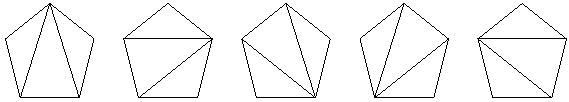
\includegraphics{cat-1}}
\пункт Сколькими способами можно правильно расставить
в ряд $n$ открывающих и $n$ закрывающих скобок?

\centerline{\texttt{a(b(cd)) \ \ \ (ab)(cd) \ \ \ ((ab)c)d \ \ \ a((bc)d) \ \ \ (a(bc))d}}
\vspace*{1mm}

\пункт Сколько путей из точки $(0,0)$ в точку $(n,n)$ идут по линиям
клетчатой бумаги вверх и вправо, не поднимаясь
выше прямой $y=x$?

\vspace*{1mm}
\centerline{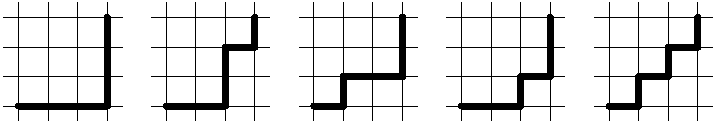
\includegraphics{cat-2}}

\пункт Сколько существует последовательностей длины $2n$, в которых $n$ раз
встречается $1$, $n$ раз встречается $-1$, и все частичные
суммы (то есть суммы нескольких (одного, двух, трёх, \dots) первых членов) %\footnote{$k$\д ой частичной суммой последовательности
%$a_1,\dots,a_p\ (k\le p)$ называется $a_1+\dots+a_k$}
неотрицательны?

\vspace*{1mm}
\centerline{\texttt{1 1 1 {-1} {-1} {-1} \ \ \ 1 1 {-1} 1 {-1} {-1}\ \ \ 1 {-1} 1 1 {-1}
{-1}\ \ \ 1 {-1} 1 {-1} 1 {-1}\ \ \ 1 1 {-1} {-1} 1 {-1}}}
\vspace*{1mm}

\пункт
На окружности даны $2n$ точек.
Сколькими способами их можно соединить $n$ непересекающимися~\hbox{хордами?}

\centerline{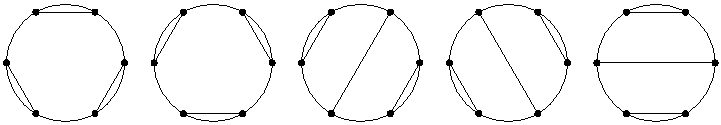
\includegraphics{cat-3}}

\пункт Найдите явную формулу для последовательности $(c_n)$, заданной
начальным условием
$c_0=1$
и рекуррентной формулой $c_{n+1}=c_0c_{n}+c_1c_{n-1}+\ldots+c_{n}c_0$
(при $n\geq0$). Вычислите $c_1,$ $c_2$, \dots, $c_5$.
\кзадача


%\задача
%Найдите первые пять чисел Каталана.
%кзадача

\задача
Найдите явные взаимно однозначные соответствия между множествами из задач
14~а,~б,~в,~г,~д.
%можно только аб, потому что б=в=г=д очевидно
\кзадача



\vfill
\ЛичныйКондуит{0mm}{6mm}

%\GenXMLW


\end{document}
